\documentclass{fkssolpub}

\usepackage[czech]{babel}
\usepackage{fontspec}
\usepackage{fkssugar}
\usepackage{amsmath}
\usepackage{graphicx}

\author{Ondřej Sedláček}
\school{Gymnázium Oty Pavla} 
\series{2j}
\problem{4} 

\begin{document}

\begin{figure}[h!]
	\centering
	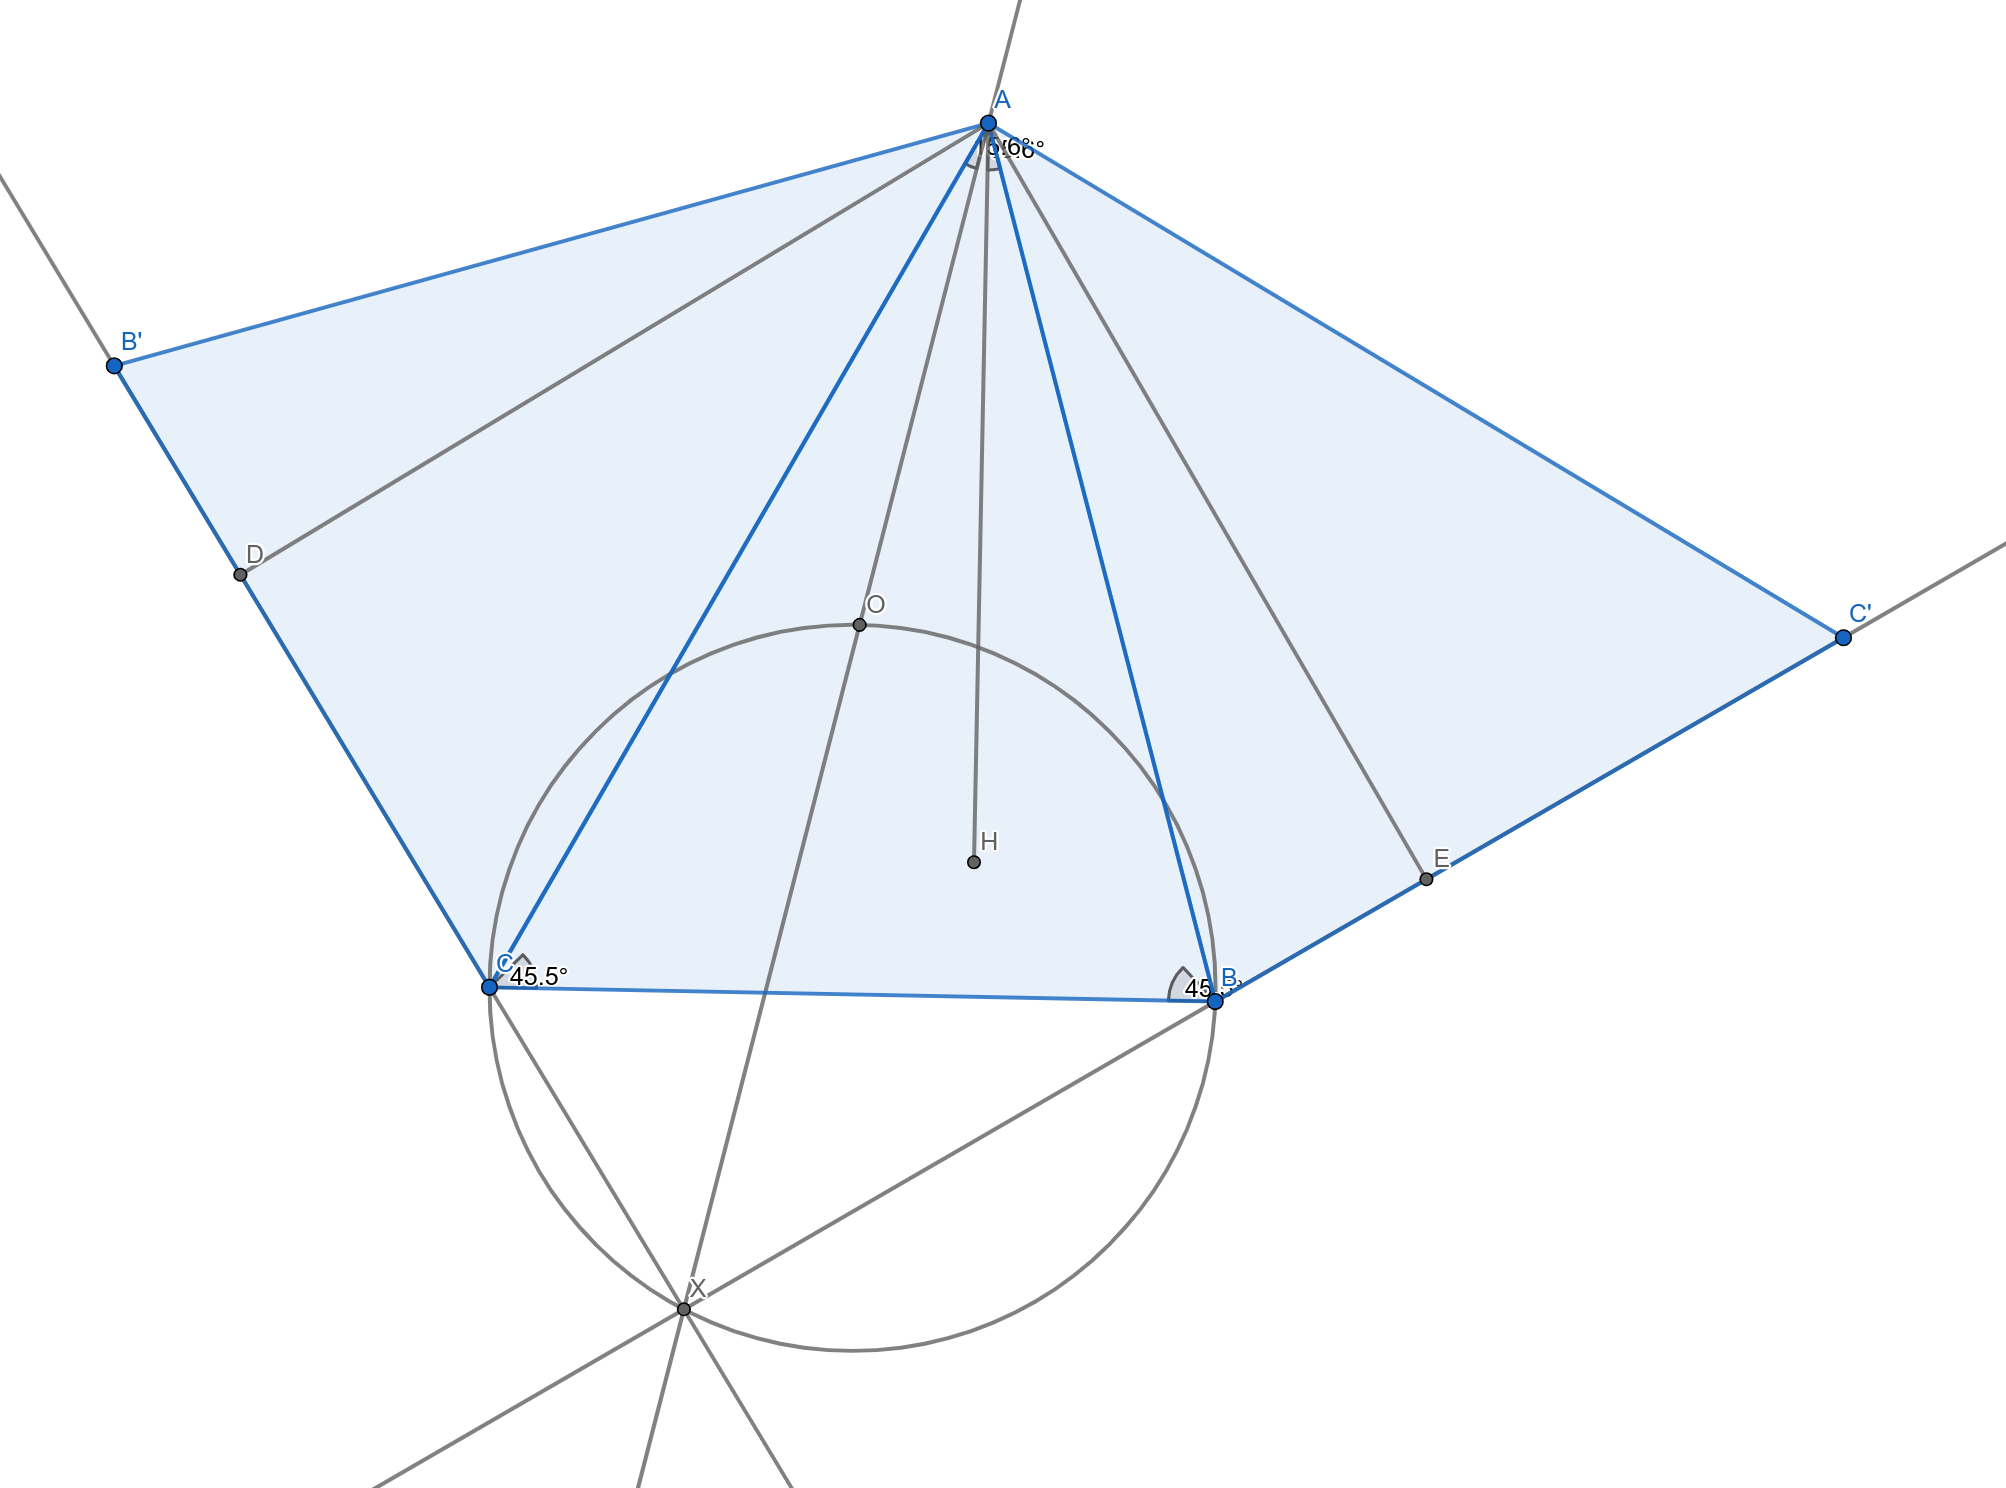
\includegraphics[width=0.6\textwidth]{4-fig1.png}
	\caption{Případ pro ostroúhlý trojúhelník}
	\label{fig:1}
\end{figure}


\begin{figure}[h!]
	\centering
	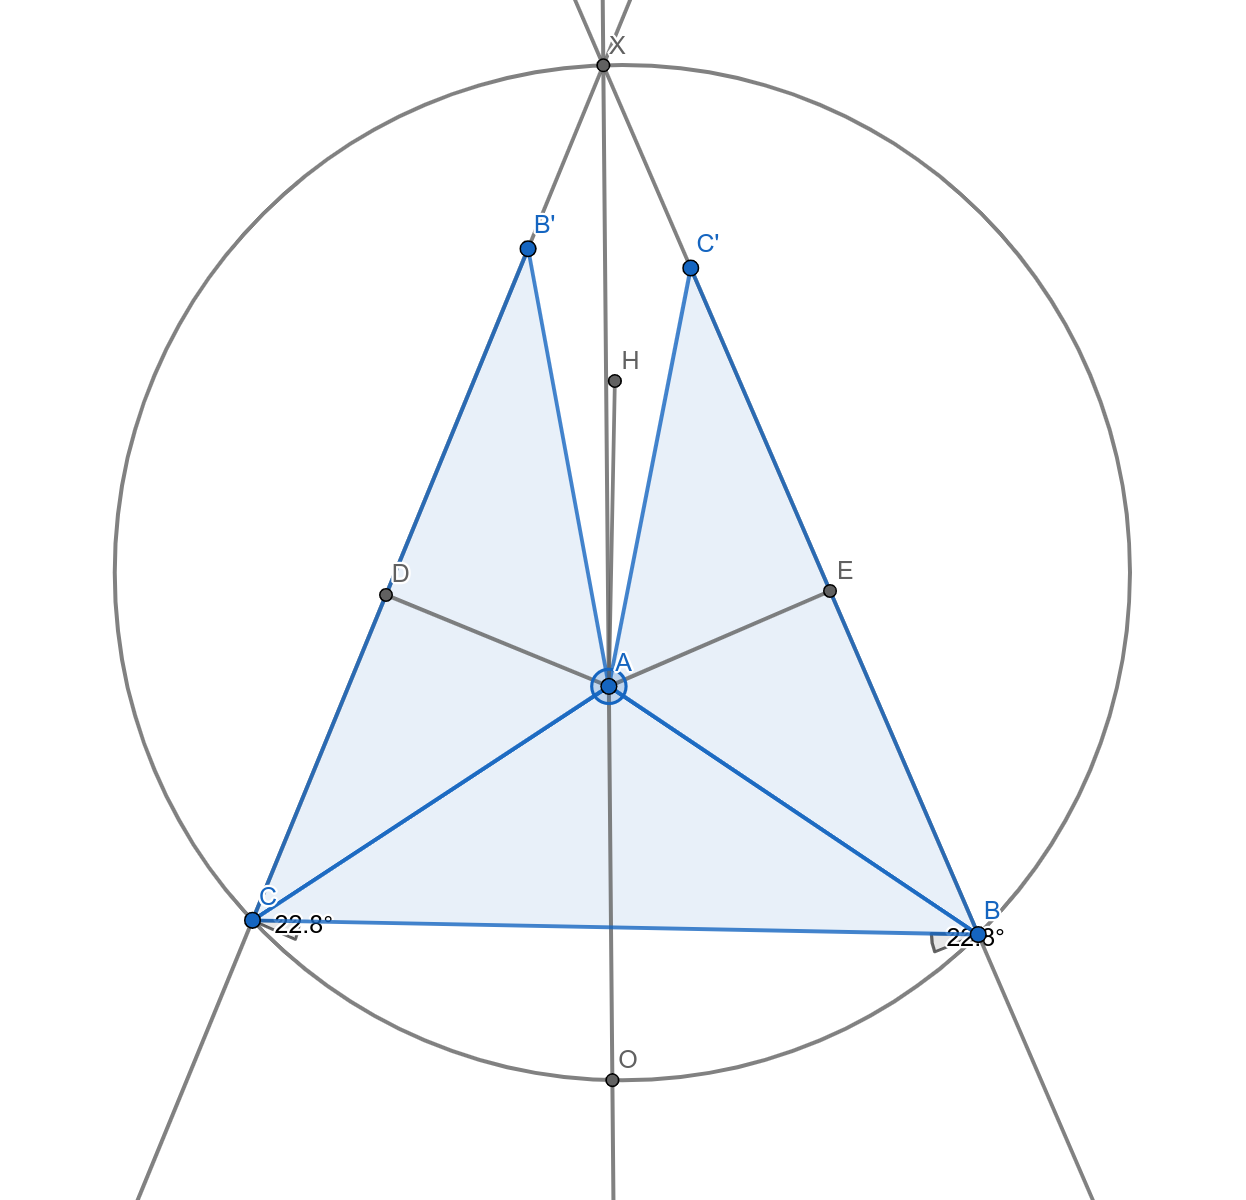
\includegraphics[width=0.6\textwidth]{4-fig2.png}
	\caption{Případ pro tupoúhlý trojúhelník s tupým úhlem u $A$}
	\label{fig:2}
\end{figure}

Jako první si dokážeme, že $A$ nutně leží na ose úhlu $\angle BXC$ nebo
na ose jeho vedlejšího úhlu. Díky projekci bodů $B'$ jsou trojúhelníky $ABC$ a
$AB'C$ shodný, stejně tak jsou shodný i
$ABC$ a $ABC'$. Tím pádem je z bodu $A$ na přímky $C'B$ a $BC'$ stejné výšky,
proto tedy nutně bod $A$ leží na ose úhlu.

Teď musíme tedy dokázat, že $O$ leží na ose úhlu $\angle BXC$. Pro dokázání
tohoto tvrzení rozdělíme na tři případy -- ostroúhlý trojúhelník, tupoúhlý s
tupým úhlem u $A$ a tupoúhlý s tupým úhlem u $B$ nebo $C$. U všech případů
dokážu, že body $B, O, C, X$ leží na jedné kružnici.

První dva se liší jen výpočtem úhlu $|\angle BXC|$, který ale vyjde
stejně:

\[
	|\angle BXC| = 180^{\circ} - |\angle CBX| - |\angle XCB|
	= 180^{\circ} - (180^{\circ} - 2 \beta) - (180^{\circ} - 2 \gamma)
	= 2 \beta + 2 \gamma - 180^{\circ}
\]
\[
	|\angle BXC| = 180^{\circ} - |\angle CBX| - |\angle XCB|
	= 180^{\circ} - 2 \beta - 2 \gamma
\]

Velikost úhlu $|\angle BOC|$ zjistíme pro první, resp. druhý případ:

\[
	|\angle BOC| = 2 \alpha
\]

\[
	|\angle BOC| = 360^{\circ} - 2\alpha
\]

Po sečtení nám pak vyjde, že $|\angle BXC| + |\angle BOC| = 180^{\circ}$,
tedy body $B, O, C, X$ leží na jedné kružnici. A protože bod $O$ leží
na ose strany $BC$, platí $|\angle CBO| = |\angle BCO|$ a tedy
$|\angle BXO| = |\angle OXC|$, což jsme chtěli ukázat.

\begin{figure}[h!]
	\centering
	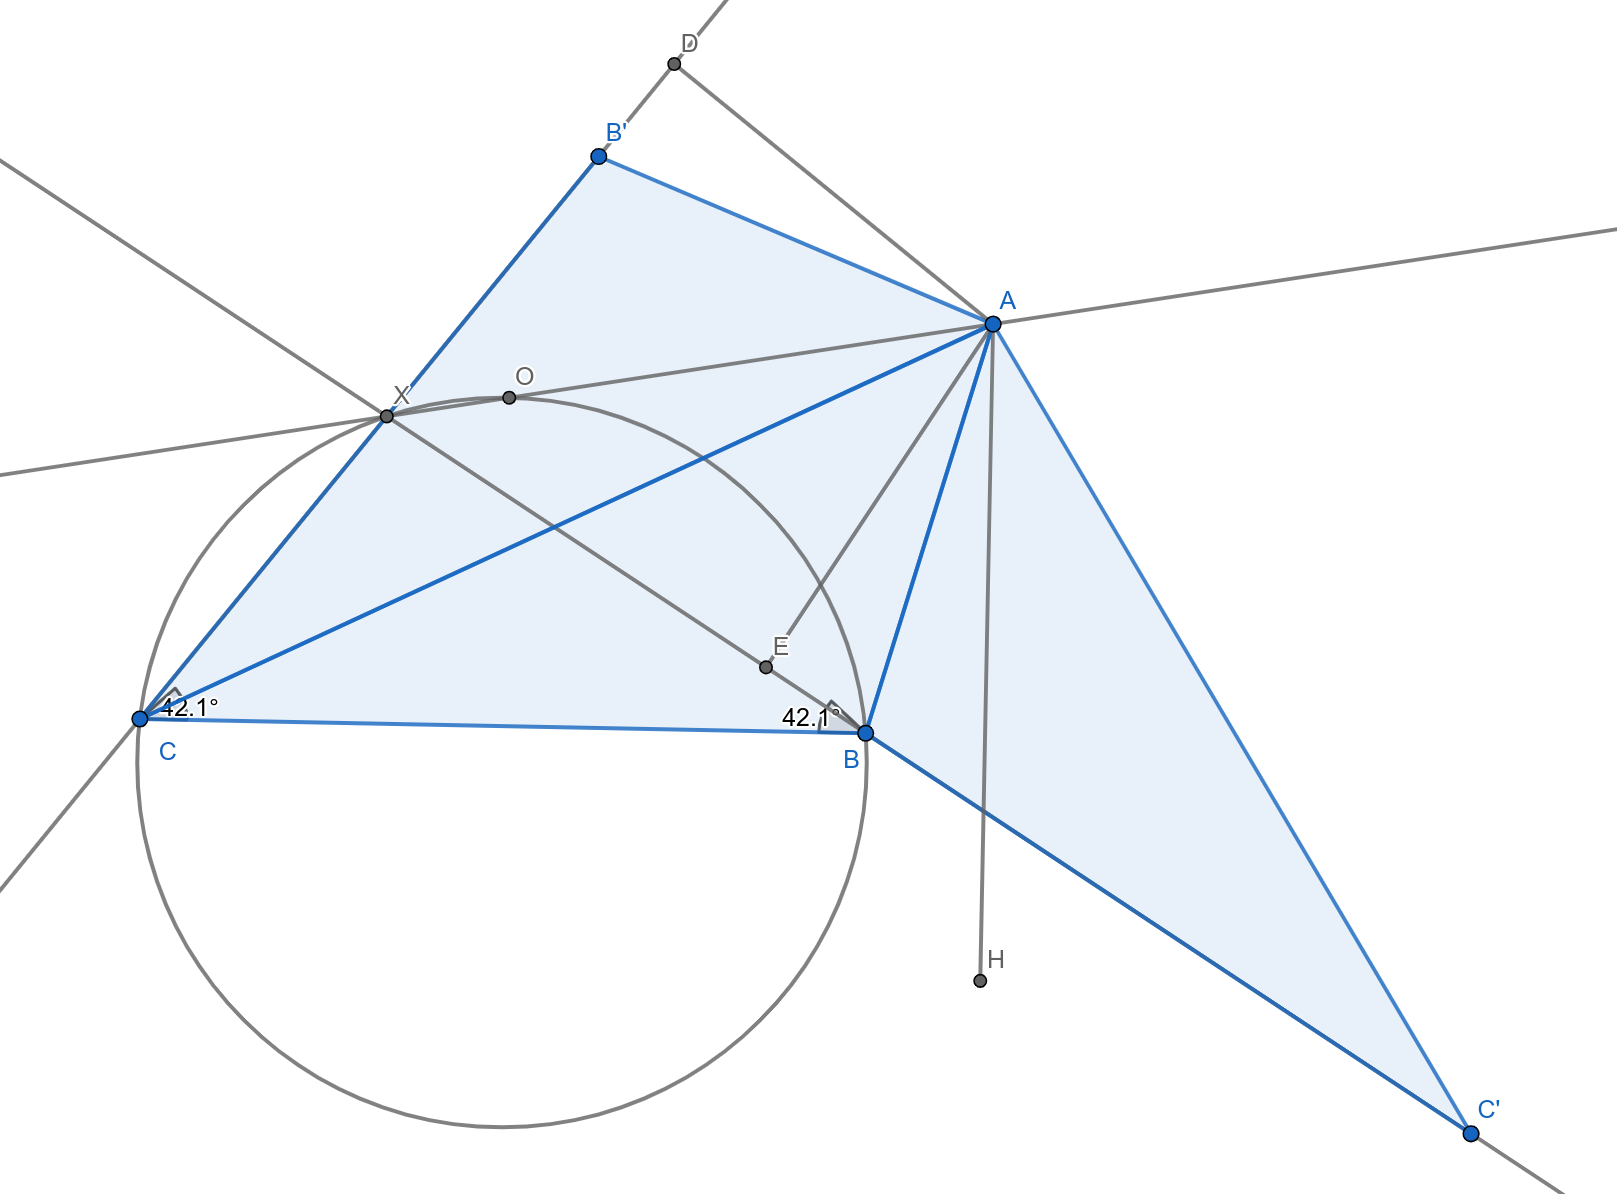
\includegraphics[width=0.6\textwidth]{4-fig3.png}
	\caption{Případ pro tupoúhlý trojúhelník s tupým úhlem u $B$ nebo $C$}
	\label{fig:3}
\end{figure}

Zbývá nám tedy poslední případ, tedy případ, kdy tupý úhel je u vrcholu $B$ nebo
$C$. Znova vypočítáme velikost úhlu při bodu $X$:

\[
	|\angle BXC| = 180^{\circ} - (2 \beta + 2 \gamma - 180^{\circ})
	= 360^{\circ} - 2 \beta - 2 \gamma
\]

Velikost středového úhlu je:

\[
	|\angle BOC| = 2 \alpha = 360^{\circ} - 2 \beta - 2 \gamma
\]

Vidíme, že v tomto případě platí $|\angle BOC| = |\angle BXC|$, tudíž se
změnilo pořadí bodů $B, C, O, X$. Musíme si proto uvědomit, že v tomto případě
leží bod $O$ na ose úhlu $\angle CXC'$. Zde úhlu $\angle CXO$ a $\angle OXC'$
dopočítáme následovně:

\[
	|\angle CXO| = |\angle CBO| = \frac{180^{\circ} - |\angle BOC|}{2}
\]
\[
	|\angle OXC'| = 180^{\circ} - |\angle OXC| - |\angle BXC| = 180^{\circ}
	- \frac{180^{\circ} - |\angle BOC|}{2} - |\angle BOC|
	= \frac{180^{\circ} - |\angle BOC|}{2}
\]

Dokázali jsme tedy zadání pro všechny případy. Tím je důkaz u konce.




\end{document}
